One of the main objectives of \sys run-time is to restrict virtual tasks to interface only with the volatile memory\todo{Do we define what a virtual task is and why is it important?}{Amjad/Sinan}, since volatile memory access is relatively cheaper than non-volatile memory access, as we already have shown experimentally in Section~\ref{section:background_task_computing} (Problem 1, Figure~\ref{fig:framEnergy}). Before dwelling into the details of virtualization of \sys, we need to shed more light on the rationale behind our approach.

\subsection{Memory Virtualization versus Intermittence}
\label{sec:virtualization_problems}

The persistent variables a virtual task operates on should be brought from non-volatile memory to a fixed-sized \emph{volatile buffer}. When the virtual task is finished the modified variables in this buffer should be committed back to their original locations in non-volatile memory. We list three fundamental problems proving that this is however a non-trivial task. 

\begin{figure}
	\centering
	%\includegraphics[width=\columnwidth]{figures/}
	\caption{\sys memory virtualization architecture.\todo{Decide if we really need this figure (we already have a lot of figs)}{Brandon}}
	\label{fig:virtualization_architecture}
\end{figure}

%\begin{figure}[t]
%	\centering
%	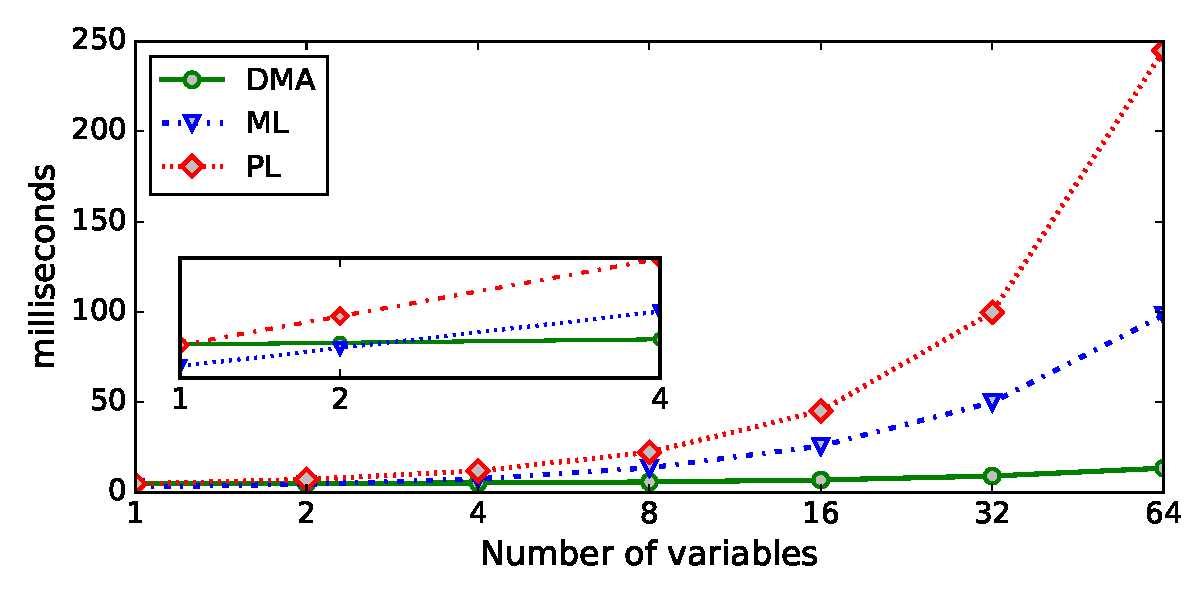
\includegraphics[width=\columnwidth]{figures/iposCommitSize}
%	\caption{Commit size delay for three memory access methods.}
%	\label{fig:virtOperationalBuf}
%\end{figure}

\textbf{Problem 1---Dynamic Access Overhead:} The persistent variables accessed and/or modified by a virtual task might not be known in advance due to the dynamic program flow. Therefore, the volatile buffer should keep track of the persistent variables accessed by any virtual task at runtime. When a persistent variable is read or written, first the volatile copy of the corresponding variable is \emph{searched} in this buffer. If it is found, the read or write operation is performed on the volatile copy. Otherwise, the persistent variable is read from the non-volatile memory and inserted in this buffer for future operations. Unfortunately, we observed that \emph{search--bring} operations at each access to the persistent variables introduce considerable overhead and might kill the benefit of task virtualization.\todo{How to show it experimentally?}{Sinan} %refer to Figure~\ref{fig:virtOperationalBuf} for experimental evaluation.

\begin{figure}[t]
	\centering
	\subfloat[SRAM Double Buffer Copy]{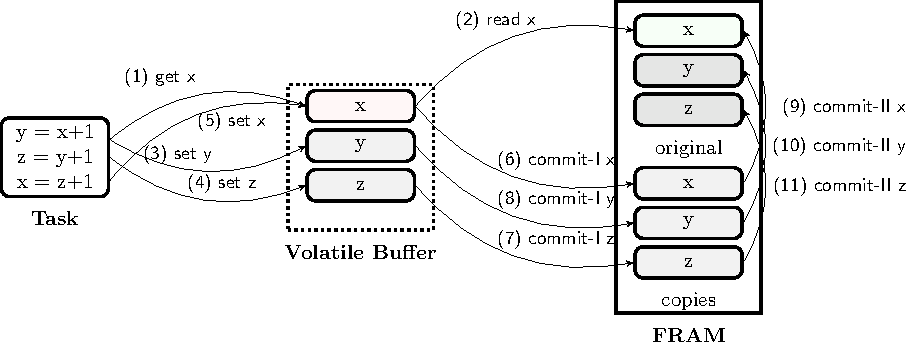
\includegraphics[width=0.49\columnwidth]{figures/sram-buffer} }
	\subfloat[DMA Copy]{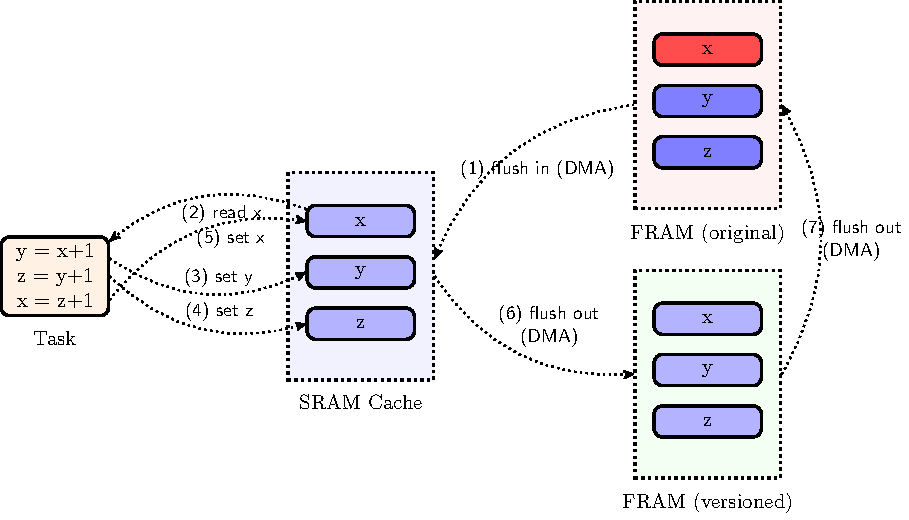
\includegraphics[width=0.49\columnwidth]{figures/dma}}
	\caption{.\todo{Explain HW/SW setup; make fonts larger, unify legends and axes}{Amjad}}
	\label{fig:sram_vs_dma}
\end{figure}

\textbf{Problem 2---Two Phase Commit Overhead:} For the consistency of the non-volatile memory, the volatile buffer should be committed at the end of each virtual task by means of a \emph{two-phase commit} approach. However, two-phase commit is also very expensive since the committed variables are not \emph{contiguous}---leading the fact that copying or moving of data between/within volatile and non-volatile memory should be always performed with CPU intervention, refer to Fig.~\ref{fig:sram_vs_dma}.

\begin{figure}[t]
	\centering
	\subfloat[Time needed to transfer a block of data]{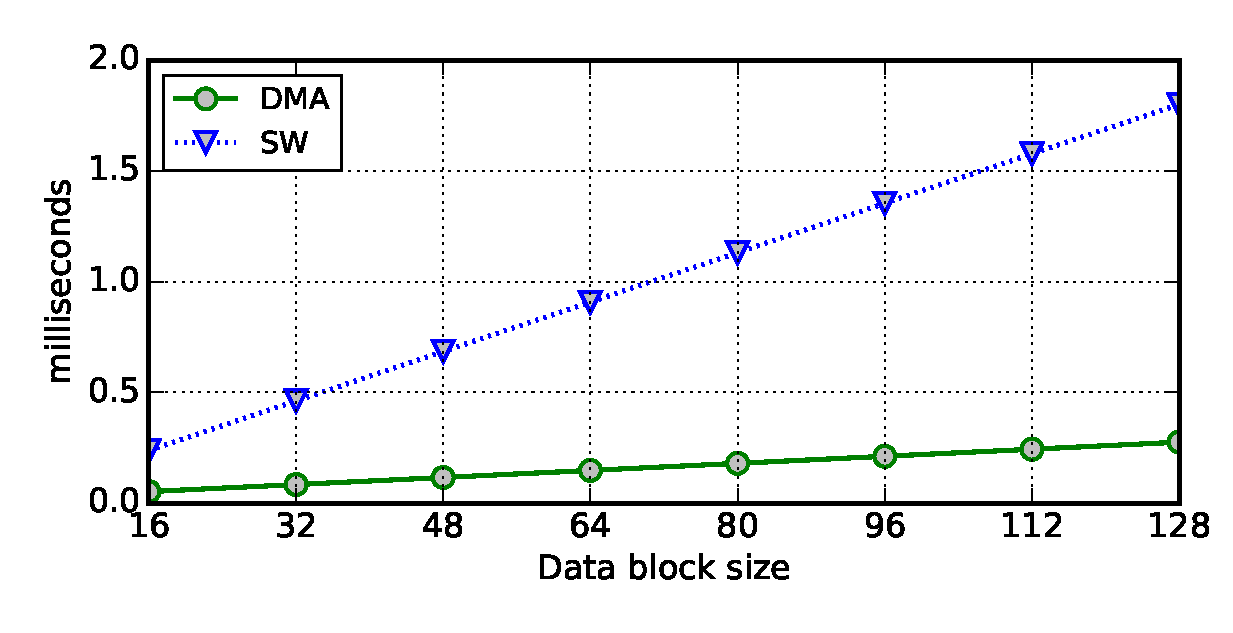
\includegraphics[width=0.49\columnwidth]{figures/dmaSize_time.eps} }
	\subfloat[Energy needed to transfer a block of data]{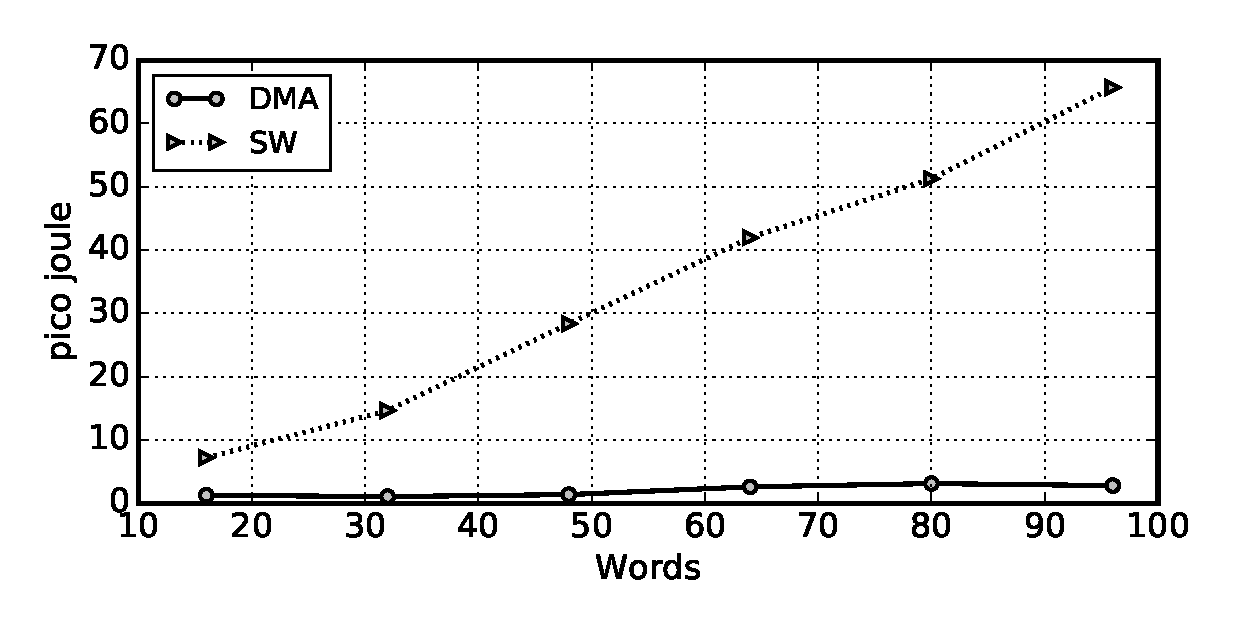
\includegraphics[width=0.49\columnwidth]{figures/energyConsumptionDMA_SW.eps}}
	\caption{Time and energy consumption of moving a block of data from SRAM to FRAM: pointers versus Direct Memory Access (DMA).\todo{Explain HW/SW setup; make fonts larger, unify legends and axes}{Amjad}}
	\label{fig:dmaTimeEnergy}
\end{figure}

\textbf{Problem 3---Main Memory Constraints:} Persistent variables can be allocated \emph{contiguously} in non-volatile memory with compiler support. In order to eliminate run-time buffer \emph{search} overhead (by not relying on specialized hardware such as e.g. in~\cite{hicks_isca_2017}), \emph{all} persistent variables can be brought from non-volatile memory to the volatile buffer at system start-up---very efficiently and faster thanks to Direct Memory Access (DMA) that eliminates CPU intervention for \emph{block} memory-memory copy/move operations, as shown experimentally in Figure~\ref{fig:dmaTimeEnergy}. Two-phase commit is also very efficient in this case since DMA can be utilized to move volatile buffer as a block to non-volatile locations. However, bringing all persistent variables from non-volatile memory to the volatile buffer suffers from the \emph{memory fit problem}: the volatile memory is a scarce resource and may not be large enough to hold all persistent variables.

Considering these facts, \sys implements a \emph{paging-based} virtual memory in software that (i) partitions contiguously allocated persistent variables into pages; (ii) implements the volatile \emph{page buffer} that holds a single page---solves the aforementioned memory-fit problem; (ii) swaps the page in volatile memory with a new page in non-volatile memory efficiently by utilizing DMA-based memory block-copy operations; (iii) buffers the swapped volatile page until commit to enable task virtualization; (iv) implements two-phase commit of the modified pages to preserve the consistency of non-volatile memory; (v) and performs two-phase commit operations using DMA for the sake of efficiency. We explain the details of \sys virtualization design in the following sections.

\subsection{Address Translation and Variable Access}

Our virtual memory system provides an interface to the applications which is composed of two C macros: \texttt{RVAR(var)} and \texttt{WVAR(var,val)} that accept the name of the persistent variable \texttt{var} as an input argument. These macros obtain the \emph{physical address} of the corresponding persistent variable in non-volatile memory and translates it into the \emph{virtual address} in volatile memory which is composed of a \emph{page tag} and \emph{offset}. For the sake of simplicity and efficiency, we implemented this translation in a trivial way: the first byte of the physical address is considered to be the page tag and the rest is the offset within the corresponding page. 

\begin{figure}
	\centering
	%\includegraphics[width=\columnwidth]{figures/}
	\caption{Address translation.\todo{Draw figure}{Sinan}}
	\label{fig:address-translation}
\end{figure}

\begin{algorithm}[t]
	\caption{\texttt{RWAR(var)} pseudo-code}
	\label{algo:rwar}
	\scriptsize
	%\small
	\begin{algorithmic}[1]
		\State $\texttt{tag}\leftarrow \texttt{getTag(var)}$ 
		\If { \texttt{tag} != \texttt{CrntPagTag} }	\Comment{Check if the page is in page buffer}
		\State	\texttt{PageFault(tag)} \Comment{Page is not in the page buffer, bring it}
		\EndIf
				\State $\texttt{offset}\leftarrow \texttt{getOffset(var)}$ 		
		\State \texttt{return pageBuf[offset]}  \Comment{Return directly from page buffer}
	\end{algorithmic}
\end{algorithm}

After address translation and obtaining the virtual address, it is required to check if the corresponding page is already in volatile page buffer. To this end, our system maintains a \texttt{CrntPagTag} variable that holds the tag of the page currently in the page buffer. If the tag of the virtual address and \texttt{CrntPagTag} are equal, this indicates that page buffer holds the required page and the offset of the virtual address is used to read from/write to the location in the volatile page buffer immediately. If the required page is not in the page buffer, a \emph{page fault} routine is executed as we discuss in the next subsection. Observe that the computational complexity of the whole steps pertaining to address translation and variable access is $\mathcal{O}(1)$---introducing minimal overhead to the system to boost up benefits of volatile-only memory interfacing. The pseudo-code of \texttt{RWAR} is presented in Algorithm~\ref{algo:rwar}.

\subsection{Page Faults and Swapping}

\todo{Section to be expanded}{Sinan}

\begin{algorithm}[t]
	\caption{\texttt{PageFault(tag)} pseudo-code}
	\label{algo:pagefault}
	\scriptsize
	%\small
	\begin{algorithmic}[1]
		\If { \texttt{isModified(CrntPagTag)} }	\Comment{Check if the active page modified}
		\State commit current page to \texttt{pagesTemp}
		\EndIf
		\If { tag is in \texttt{pagesTemp} }	\Comment{Check if the requested page has been modified}
		\State bring from \texttt{pagesTemp} to \texttt{pageBuff} 
		\Else
		\State bring from original to \texttt{pageBuff} 
		\EndIf 
	\end{algorithmic}
\end{algorithm}

If the tag of the virtual address and \texttt{CrntPagTag} are not equal, the active page in page buffer should be swapped with the requested page. In this situation, we have the following two cases:

\paragraph{Modified Active Page:} If the contents of the page buffer is modified, we commit it to an intermediate page buffer in non-volatile memory, namely to \texttt{pagesTemp}. If it is not modified, there is no need to commit the active page.

\paragraph{Modified Requested Page:}  If the requested page is previously modified, it should be brought from \texttt{pagesTemp} rather than its original location in non-volatile memory. 

After the swapping, the \texttt{CrntPagTag} is set to the tag of the requested page. It should be noted that DMA is used to introduce minimal overhead during page swapping. The pseudo-code of the page fault handling is presented in Algorithm~\ref{algo:pagefault}.

\subsection{Page Committing}

Using a two-phase commit by utilizing DMA. \todo{Text to be written}{Sinan}

%%% Old Text by Amjad %%%

%\begin{algorithm}[t]
%	\caption{Virtualized Operational Buffer}
%	\label{algo:virtuBufWrite}
%	\scriptsize
%	%\small
%	\begin{algorithmic}[1]
%		\State $var \in \text{\{global variables\}} $ 
%		\State \label{lst:virtuBufWrite:line:begin}\Call{Virtual Task()}{} 
%		\While { \textit{executing} } \Comment{Execution stage}
%		\State $var$  $\rightarrow$ \textsf{volatile buffer} \label{lst:virtuBufWrite:line:output}
%		\If { $var$  in \textsf{ volatile buffer} }				\label{lst:virtuBufWrite:line:inputBegin}
%		\State $var$  $\leftarrow$  \textsf{volatile buffer} 
%		\Else 
%		\State $var$  $\leftarrow$  \textsf{FRAM}		\label{lst:virtuBufWrite:line:inputEnd}
%		\EndIf
%		
%		\If {power interrupts}
%		\State back to \ref{lst:virtuBufWrite:line:begin}
%		\EndIf
%		\EndWhile
%		
%		\While{  $\textsf{volatile buffer}\not=\emptyset$  } \label{lst:virtuBufWrite:line:commitBegin} \Comment{ First phase commit}
%		\State \textsf{volatile buffer} $\rightarrow$  \textsf{persistent buffer}
%		\If {power interrupts}
%		\State discard \textsf{persistent buffer}
%		\State back to  \ref{lst:virtuBufWrite:line:begin} 
%		\State   \label{lst:virtuBufWrite:line:commitEnd}
%		\EndIf
%		\EndWhile 
%		
%		\While{ $\textsf{persistent buffer}\not=\emptyset$ } \label{lst:virtuBufWrite:line:SecCommitBegin} \Comment{Second phase commit}
%		\State \textsf{persistent buffer} $\rightarrow$ FRAM 
%		\If {power interrupts}
%		\State Continue
%		\EndIf
%		\EndWhile 
%		\State     \label{lst:virtuBufWrite:line:SecCommitEnd}
%		\State return
%	\end{algorithmic}
%\end{algorithm}

%Since accessing FRAM is more energy expensive and slower than accessing SRAM, preventing frequent access to FRAM (i.e. during looping operations) is desirable. Therefore, the first proposed protection method utilizes a volatile buffer that holds temporary all the outputs of a virtual task (see Algorithm~\ref{algo:virtuBufWrite} line~\ref{lst:virtuBufWrite:line:output}). Consequently, a virtual task must first attempt to read a global variable from the volatile buffer before trying to obtain the value from the non-volatile memory (see Algorithm~\ref{algo:virtuBufWrite} lines~\ref{lst:virtuBufWrite:line:inputBegin}-\ref{lst:virtuBufWrite:line:inputEnd}) to ensure a correct execution progress and the consistency of the memory. Once the execution of a virtual task is done, the first phase of the commit process is started by copying the volatile buffer to a persistent buffer (see Algorithm~\ref{algo:virtuBufWrite} lines~\ref{lst:virtuBufWrite:line:commitBegin}-\ref{lst:virtuBufWrite:line:commitEnd}). If the power is interrupted the persistent buffer must be discarded and the execution must start again from the beginning of the virtual task. In another words, the first phase commit must be performed atomically to preserve the consistency of the output of a virtual task. The second phase commit is a power failure immune precess that is responsible for distributing the global variables to their final locations and make the non-volatile memory consistent and synchronized with the computation progress (see Algorithm~\ref{algo:virtuBufWrite}lines~\ref{lst:virtuBufWrite:line:SecCommitBegin}-\ref{lst:virtuBufWrite:line:SecCommitEnd}).

%\paragraph{Virtualized Operational Buffer: Implementation} 

%We implement a reference implementation of \sys that uses virtualized Operational buffer to protect the data against power failure. 

%\paragraph{Virtual Buffer}

%We realized the virtaulzed buffer as a volatile hashed table of linked lists. The hashing technique was chosen to reduce the buffer searching time and the linked lists are used to prevent data loss when there is a conflict between multiple variables---If two variables have the same hash value they will occupy the same cell, however, with linked list a new node will be created for each variable to resolve the conflict and protect the data. The hashing function is based on the observation that the virtual addresses of the memory cells have approximately a flat distribution over the memory addressing space and the fact that each entry, of the virtual table, has the address and the value of a variable. As such, by using the least significant bits as an index to access the virtual buffer the hash function distributes its inputs uniformly in the virtual buffer. Accordingly, the linked lists search time, on average, is reduced. 

%Despite the fact that the linked lists reduce the average complexity of searching the virtual buffer significantly, they introduce a number of drawbacks: (i) the linked list data structure introduce a non-negligible memory overhead while it relies on a limited memory section, namely the heap; (ii) traversing the linked list is relatively slow. Therefore, we re-implemented the virtual buffer, after observing that most of the global variables have the same most significant bits, as a bigger hashed table that does not allow entries conflict. To eliminate the need for searching the hashed table linearly while committing its entries, we add a new buffer that holds the indices of the occupied cells of the hashed table. This table is of the same length as the hashed table. We can reason about the benefit of this buffer as follows: if we assume that the global variables are evenly divided between the tasks, then this buffer reduces the commit time by a factor equal to the number of tasks.   

%\paragraph{Persistent Buffer}

%The persistent buffer is implemented as static array of tuples, where each tuple holds  the address and the value of a variable. This data structure is very suitable for the second phase commit where each element has to be committed to its finial location. However, the complexity of committing this buffer is of size $O(N)$, where $N$ equals the length of the buffer. Therefore, the size of the buffer can have dramatic effect on the performance of \sys---On one hand, if the size of the buffer is small the buffer overflow problem will be very serious. On the other hand, if the size of the buffer is large \sys will experience a significant performance degradation. However, by observing the type of the information that this buffer holds, namely memory addresses, we can, on average, reduce the complexity of committing this buffer by defining the \emph{effective size} of the buffer to be the size of the buffer up to the first cell that holds an invalid memory address. Moreover, since this buffer is in FRAM which is much bigger than SRAM its size can be relatively big. 

% \paragraph{Virtualized Operational Buffer: delay analysis}[initial results]

% \begin{figure}[t]
% 	\centering
% 	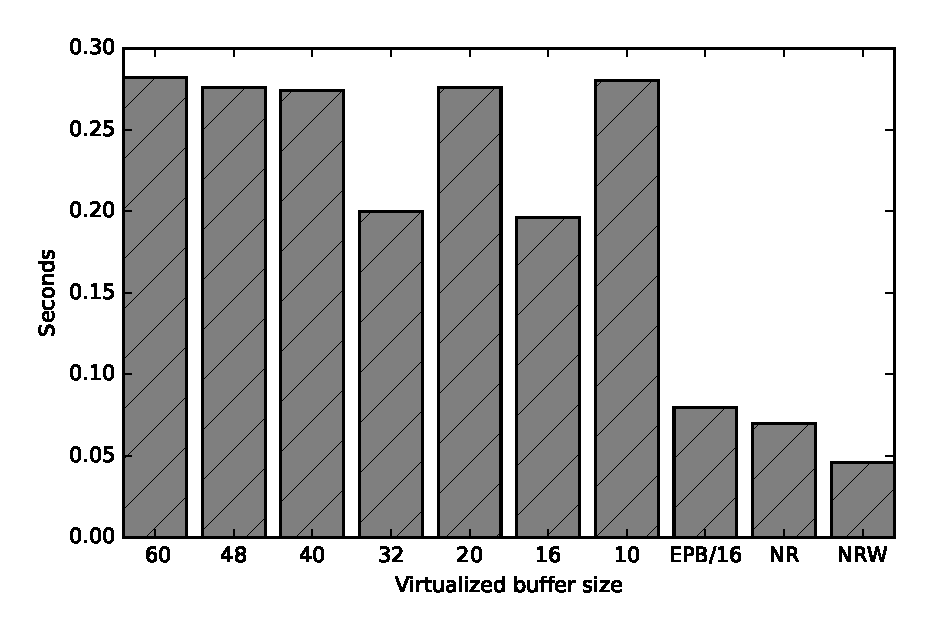
\includegraphics[width=\columnwidth]{figures/virtual_buffer_size.eps}
% 	\caption{\sys based on virtualized Operational Buffer. It runs the decompression application with different buffer configurarions. EPB: Enhanced Persistent Buffer. NR: no read operation from the buffer. NRW: not read or write operations from the buffer.}
% 	\label{fig:virtOperationalBuf}
% \end{figure}

% 	To analyze the performance of \sys versus the sizes of the virtual buffer and the persistent buffer we setup the following experiment. We let IPOS to run the decompression application---until the data decompression is completely finished---and we capture the execution time using a logic analyzer~\cite{xxx}. The results presented in Fig.~\ref{fig:virtOperationalBuf} show the \sys has its best performance when the virtual buffer size is 16, where the execution time was $\approx$196 ms. 

% 	All the experiments were done with a persistent buffer of size 100. However, the bar labeled with "EPB/16" in  Fig.~\ref{fig:virtOperationalBuf} shows the effect of the enhanced commit process that uses the buffer effective size instead of the buffer maximum size. We see that the execution time is reduced to $\approx$80 ms. Furthermore, we quantized the overhead of the read operations from the buffer, by eliminating this operation, and the bar labeled with "NR" shows that it cost  $\approx$10 ms. Moreover, the overhead of the read and write operations is $\approx$34 ms as compared to \sys best performance, see the bar labeled with "NRW" in Fig.~\ref{fig:virtOperationalBuf}. 